\documentclass[a4paper,10pt,ngerman]{scrartcl}
\usepackage{babel}
\usepackage[T1]{fontenc}
\usepackage[utf8x]{inputenc}
\usepackage[a4paper,margin=2.5cm,footskip=0.5cm]{geometry}

% Die nächsten drei Felder bitte anpassen:
\newcommand{\Aufgabe}{Aufgabe 1: Weniger krumme Touren} % Aufgabennummer und Aufgabennamen angeben
\newcommand{\TeilnahmeId}{65336}                  % Teilnahme-ID angeben
\newcommand{\Name}{Philip Gilde}             % Name des Bearbeiter / der Bearbeiterin dieser Aufgabe angeben

% Kopf- und Fußzeilen
\usepackage{scrlayer-scrpage, lastpage}
\setkomafont{pageheadfoot}{\large\textrm}
\lohead{\Aufgabe}
\rohead{Teilnahme-ID: \TeilnahmeId}
\cfoot*{\thepage{}/\pageref{LastPage}}

% Position des Titels
\usepackage{titling}
\setlength{\droptitle}{-1.0cm}

% Für mathematische Befehle und Symbole
\usepackage{amsmath}
\usepackage{amssymb}

% Für Bilder
\usepackage{graphicx}

% Für Algorithmen
\usepackage{algpseudocode}
\usepackage{amsthm}
\usepackage{tabularx}
\usepackage{booktabs}

% Für Quelltext
\usepackage{listings}
\usepackage{color}
\definecolor{mygreen}{rgb}{0,0.6,0}
\definecolor{mygray}{rgb}{0.5,0.5,0.5}
\definecolor{mymauve}{rgb}{0.58,0,0.82}
\lstset{
  keywordstyle=\color{blue},commentstyle=\color{mygreen},
  stringstyle=\color{mymauve},rulecolor=\color{black},
  basicstyle=\footnotesize\ttfamily,numberstyle=\tiny\color{mygray},
  captionpos=b, % sets the caption-position to bottom
  keepspaces=true, % keeps spaces in text
  numbers=left, numbersep=5pt, showspaces=false,showstringspaces=true,
  showtabs=false, stepnumber=2, tabsize=2, title=\lstname
}
\lstdefinelanguage{JavaScript}{ % JavaScript ist als einzige Sprache noch nicht vordefiniert
  keywords={break, case, catch, continue, debugger, default, delete, do, else, finally, for, function, if, in, instanceof, new, return, switch, this, throw, try, typeof, var, void, while, with},
  morecomment=[l]{//},
  morecomment=[s]{/*}{*/},
  morestring=[b]',
  morestring=[b]",
  sensitive=true
}

% Diese beiden Pakete müssen zuletzt geladen werden
%\usepackage{hyperref} % Anklickbare Links im Dokument
\usepackage{cleveref}

% Daten für die Titelseite
\title{\textbf{\Huge\Aufgabe}}
\author{\LARGE Teilnahme-ID: \LARGE \TeilnahmeId \\\\
  \LARGE Bearbeiter/-in dieser Aufgabe: \\
  \LARGE \Name\\\\}
\date{\LARGE\today}
\newtheorem{theorem}{Satz}
\newtheorem{lemma}[theorem]{Lemma}
\begin{document}

\maketitle
\tableofcontents

\vspace{0.5cm}

\section{Lösungsidee}
\subsection{Annäherung einer optimalen Lösung}
Das Problem wird mit Hilfe des Simulated Annealing \cite{kirkpatrick_1983}
gelößt.
\begin{algorithmic}
  \Procedure{Simulated Annealing}{Startlösung $S$, Temperatur $T_0$, Abkühlkoeffizient $\alpha$, Minimale Temperatur $T_{min}$}
  \State{$S_{Beste} \gets S$}
  \State{$C_{Beste} \gets C(S)$}
  \State{$T \gets T_0$}
  \While{$T > T_{min}$}
  \State{$S_{Neu} \gets \text{Nachbarlösung von } S$}
  \State{$C_{Neu} \gets C(S_{Neu}) $}
  \If{$C_{Neu} < C_{Beste}$}
  \State{$C_{Beste} \gets C_{Neu} $}
  \State{$S_{Beste} \gets S_{Neu} $}
  \EndIf
  \State{$r \gets \text{Zufallszahl aus }[0,1]$}
  \If{$r < \exp(\frac{C(S)-C_{Neu}}{T})$}
  \State{$S \gets S_{Neu}$}
  \EndIf
  \State{$T \gets \alpha T$}
  \EndWhile

  \Return{$S_{Beste}$}
  \EndProcedure
\end{algorithmic}
Die grundlegende Idee des Algorithmus ist, das Problem als ein sich abkühlendes thermodynamisches System zu modellieren,
wobei die Kosten für eine Lösung der Energie des Systems entspricht. Die Wahrscheinlichkeit, in einen anderen
Zustand überzugehen, ist dann abhängig von der Energiedifferenz. Die auch von der Temperatur abhängige Wahrscheinlichkeit
ist von der Boltzmann-Verteilung inspiriert. Das thermodynamische System befindet sich nach dem Abkühlen in einem
energiearmen Zustand, genauso sollte der Algorithmus eine möglichst kostengüstige Lösung finden. Mit $T\to 0$ handelt es sich
bei dieser Methode um einen einfachen Bergsteigeralgorithmus, der immer eine kostengüstigere benachbarte Lösung auswählt. Dieser
kann leicht in lokalen Minima stecken bleiben, also bei Lösungen, die keine besseren Nachbarn haben, aber nicht das globale Minimum sind.
Um das zu vermeiden kann Simulated Annealing durch die temperatur- und kostendifferenzabhängige Übergangswahrscheinlichkeit anfangs lokale
Minima überwinden.\\
Gültige Lösungen sind hier alle möglichen Permutationen von $N$ Landeplätzen. Die Beschränkung, dass eine
Lösung keine Spitzen Winkel beinhalten darf, wird über die Kostenfunktion $C(S)$ kodiert. Die Kostenfunktion
setzt sich zusammen aus der Länge des von $S$ gebildeten Pfades und einer Gebühr $g \in \mathbb{R}$ für jeden spitzen Winkel. $g$
ist eine obere Schranke der Länge eines Pfades, wodurch für jeden Pfad $S'$ mit weniger spitzen Winkeln als $S$
gilt $C(S) > C(S')$. Diese obere Schranke erschließt sich aus der Überlegung, dass eine mögliche Lösung mindestens $N-1$ Kanten haben muss.
Dieser Pfad kann höchstens die Kosten der teuersten $N-1$ Kanten haben. \\
Um Nachbarn einer Lösung zu finden, habe ich die für das klassische TSP bekannten Mutationsoperatoren \textbf{Insert}, \textbf{Displace}, \textbf{Reverse-Displace}
\cite{larranaga_1999}
und einen eigenen, auf dem 3-Opt-Verfahren basierenden Mutationsoperator, den ich \textbf{3-Opt} nenne, verwendet. Es wird zufällig einer der Operatoren angewendet.
Die Operatoren basieren auf der
Darstellung eines Pfades als Permutation von $(1, 2, \ldots, N)$. In dieser Darstellung gibt das $k$-te Element der Permutation
an, welcher Landeplatz als $k$-tes besucht wird.
\begin{description}
  \item[Insert] wählt einen zufälligen Landeplatz der Permutation aus und setzt ihn an
    eine zufällige neue Stelle. Wenn wir zum Beispiel die Permutation
    $(1,2,3,4,5,6)$ haben und der dritte Landeplatz ausgewählt wird, könnte die
    erzeugte Permutation $(1,2,4,5,3,6)$ sein, wenn die vorletzte als neue Position
    ausgewählt wurde.
  \item[Displace] wählt ein zufälliges Segment der Permutation aus und setzt es an eine
    zufällige neue Stelle. Wenn von der Permutation $(1,2,3,4,5,6)$ das Segment
    $(2,3,4)$ ausgewählt wird, könnte das Ergebnis $(1,5,2,3,4,6)$ sein, wenn
    wieder die vorletzte Stelle ausgewählt wurde.
  \item[Reverse-Displace] wählt ein zufälliges Segment der Permutation aus und setzt es
    in umgekehrter Reihenfolge an eine zufällige neue Stelle. Beim Beispiel aus
    \textbf{Displace} wäre das Ergebnis dann $(1,5,4,3,2,6)$.
  \item[3-Opt] teilt den Pfad an zufälligen Stellen in vier Segmente auf. Diese werden
    in einer zufälligen neuen Reihenfolge zusammengesetzt, wobei sie mit Wahrscheinlichkeit
    0.5 umgekehrt werden. Der Operator ähnelt der 3-Opt-Heuristik, welche 3 Kanten einer
    Lösung löscht und die Segmente in einer Reihenfolge zusammensetzt, welche die Gesamtkosten
    minimiert, denn er ersetzt auch 3 Kanten durch neue. Wenn von der Lösung $(1,2,3,4,5,6,7,8,9)$ die Segmente
    $(1,2)$, $(3,4)$, $(5,6)$ und $(7,8,9)$ ausgewählt werden, könnte das Ergebnis $(4,3,5,6,9,8,7,1,2)$ sein.
\end{description}
Für die Starttemperatur $T_0$ ist es sinnvoll, einen Wert zu nehmen, der Anfangs für alle Lösungen eine höhe Übergangswahrscheinlichkeit
erlaubt. Es ist sinnvoll, ein Vielfaches von $g$ zu verwenden, damit Anfangs mehrere spitze Winkel dazukommen können. \textbf{Displace}, \textbf{Reverse-Displace} und
\textbf{3-Opt} tauschen drei Kanten aus und fügen dadurch maximal sechs neue spitze Winkel hinzu. Deshalb sollte die Temperatur anfangs mindestens $7g$ betragen. Durch
Ausprobieren hat sich eine Starttemperatur von $16g$, eine Mindesttemperatur von $0.001$ und ein Abkühlkoeffizient von $0.999999$ durchgesetzt. Weiterhin war es sinnvoll, die Suche abzubrechen, wenn für
$1000000$ Iterationen keine neue beste Lösung gefunden wurde. \\
Der Algorithmus lässt sich so modifizieren, dass er möglichst schnell eine Lösung ohne spitze Winkel findet. Dafür wird einerseits ein weiteres Abbruchkriterium
eingeführt, dass sofort abbricht, wenn eine Lösung ohne spitze Winkel gefunden wurde. Andererseits wird zuerst ein recht kleiner Abkühlkoeffizient von beispielsweise
$0.5$ verwendet, wodurch potenziell weniger Iterationen notwendig sind um eine gute Lösung zu finden. Wenn das nicht ausreicht, wird der Abkühlkoeffizient erhöht und der Algorithmus
erneut ausgeführt. Das wird so lange wiederholt, bis eine sinnvolle Lösung gefunden wurde, oder eine grenze der Iterationen erreicht wurde.
\subsection{Erweiterung: Optimale Lösung}

\begin{figure}[t]
  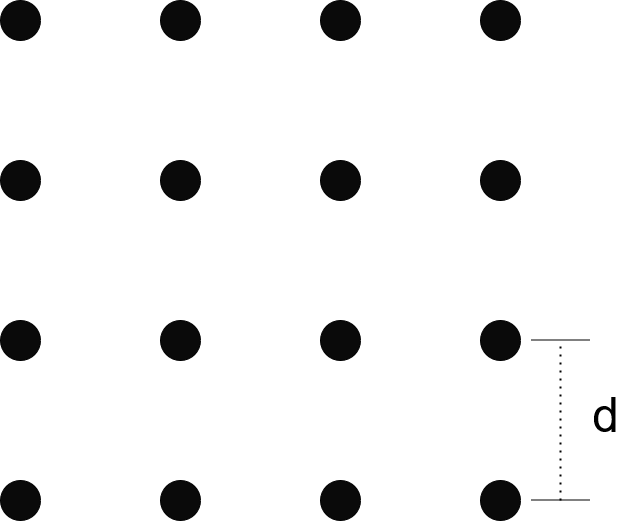
\includegraphics[scale=.2]{struktur}
  \centering
  \caption{Die 16-Struktur.}
\end{figure}
\begin{figure}[t]
  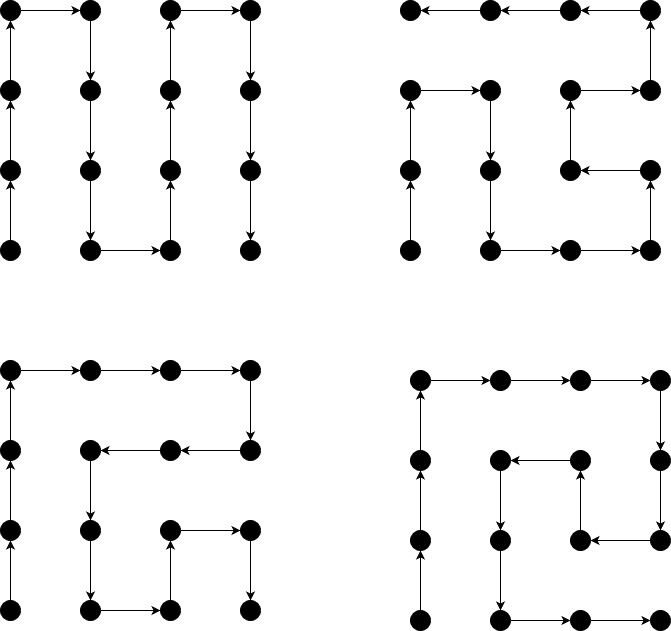
\includegraphics[scale=0.5]{richtungen}
  \centering
  \caption{Ein von unten in die 16-Struktur kommendes Flugzeug kann in alle Richtungen weiter fliegen. Für andere Herkunftsrichtungen müssen die Pfade entsprechend gedreht werden.}
\end{figure}
Es ist $\mathcal{NP}$-schwer, das weniger krumme Touren-Problem (WKT) optimal
zu lösen. Um das zu zeigen, wird eine Reduktion vom eulerschen Pfad-Problem des
Handlungsreisenden (E-PTSP) skizziert, welches $\mathcal{NP}$-schwer ist \cite{papadimitriou_1977}. E-PTSP lautet folgendermaßen: Es dei $P \subset
  \mathbb{R}^2$ eine endliche Menge. Dann wird eine Reihenfolge von P gesucht,
bei der die Strecke zwischen aufeinanderfolgenden Punkten minimal ist. \\
E-PTSP kann nun auf WKT reduziert werden, in dem jeder der Punkte $P$ durch
eine 16-Struktur an dessen Position ersetzt wird (Siehe Abbildung 1).\\
Diese Transformation heißt im folgenden $T_d: \mathfrak{P}(\mathbb{R}) \rightarrow \mathfrak{P}(\mathbb{R})$
mit $d \in \mathbb{R}$,
wobei $\mathfrak{P}$ für die Potenzmenge steht.
\begin{lemma}
  Es sei $P$ eine Instanz von E-PTSP und $P'=T_d(P)$ mit $d$ so dass sich die 16-Strukturen nicht überschneiden.
  Dann entspricht eine Permutation der 16-Strukturen von $P'$ einer Lösung von $P'$.
\end{lemma}
\begin{proof}
  Die erste 16-Struktur der Permutation kann in einer der Reihenfolgen in Abbildung 2 abgeflogen werden, so dass
  die beiden zuletzt angeflogenen Punkte in Richtung der nächsten 16-Struktur in der Permutation zeigen.
  Alle 16-Strukturen der Permutation bis auf die letzte liegen dann zwischen zwei anderen 16-Strukturen.
  Abbildung 2 zeigt, dass diese dei 16-Strukturen nacheinander angeflogen werden könne, egal wie sie zuenander
  liegen. Die letzte 16-Struktur kann dann in einer beliebigen Reihenfolge angeflogen werden.
\end{proof}
\begin{lemma}
  Es sei $P$ eine Instanz von E-PTSP.
  $P' = T_d(P)$ kann in eine mögliche Lösung von $P$ umgewandelt werden,
  wenn die Punkte jeder 16-Struktur jeweils unmittelbar nacheinander angeflogen werden.
\end{lemma}
\begin{proof}
  Jeder Punkt in $P'$ darf genau einmal besucht werden. Wenn die Punkte einer 16-Struktur
  unmittelbar nacheinander angeflogen werden, kann diese Struktur danach nicht mehr angeflogen werden.
  Dadurch wird in einer solchen Lösung jede 16-Struktur nur einmal angeflogen. Die Lösung stellt also
  eine Permutation der 16-Strukturen dar. Da jede 16-Struktur einen entsprechenden Punkt in $P$ hat,
  kann die Permutation der 16-Strukturen so in eine Permutation von $P$ umgewandelt werden.
\end{proof}
Nun sei $\lim \limits_{d \to 0}$. Die Abstände zwischen Punkten gleicher 16-Strukturen
nähert sich dann $0$ an, während die Abstände zwischen Punkten unterschiedlicher 16-Strukturen den Abständen
der entsprechenden Punkte in der E-PTSP-Instanz annähern. Die Länge eines Pfades, der die Punkte einer
16-Struktur unmittelbar nacheinander besucht, nähert sich dann der Länge des entsprechenen Pfad in der E-PTSP-Instanz an.
Es muss jetzt noch gezeigt werden, dass eine optimale Lösung die Punkte einer Struktur unmittelbar nacheinander
besucht und deshalb in eine Lösung des entsprechenden E-PTSP umgewandelt werden kann. Nach dem Beweis von
Lemma 1 ist das äquivalent mit der Aussage, dass eine optimale Lösung jede 16-Struktur nur einmal besucht.
\begin{lemma}
  Es sei $P$ eine Instanz von E-PTSP und $P'=T_d(P)$. \\
  1.
  Wenn eine mögliche Lösung $L$ 16-Strukturen mehrmals besucht,
  gibt es eine bessere oder gleichgute Lösung $L'$, die sie nur einmal besucht. \\
  2.
  $L'$ kann in polynomieller Zeit gefunden werden.
\end{lemma}
\begin{proof}
  1.
  Wir betrachten die Reihenfolge, in der $L$ die 16-Strukturen besucht. $L$ besucht $n \geq 2$ 16-Strukturen, bevor
  es eine 16-Struktur besucht, die es schon besucht hat. Wenn $n=|P|$ besucht $L$ keine 16-Strukturen mehrmals.
  Andernfalls besucht $L$ danach eine 16-Struktur, die es schon besucht hat. Diese 16-Struktur können wir überspringen,
  wodurch wir eine neue Verkettung von 16-Strukturen erhalten, in der $n$ um 1 größer ist. Nach der Dreiecksungleichung
  ist diese Verkettung kürzer als die davor. Wir erhalten so lange neue Verkettungen, bis $n=|P|$ und keine Struktur mehrmals
  besucht wird. Es handelt sich dann um eine Permutation der 16-Strukturen.\\
  2. $L'$ wird gefunden, in dem die Verkettung von 16-Strukturen $L$ durchgegangen wird und jede 16-Struktur,
  die schon einmal darin vorkam gelöscht wird. Es wird also jede der $n=|L|$ in $L$ vorkommenden
  16-Strukturen mit allen Vorangegangenen verglichen. Da es maximal $n$ vorangegangene 16-Strukturen gibt,
  haben wir $\mathcal{O}(n^2)$ Vergleiche, es ist unter der Annahme von konstanter Vergleichszeit $t \in \mathcal{O}(n^2)$.
\end{proof}
Eine optimale Lösung kann deshalb immer in eine Lösung für E-PTSP umgewandelt werden. Diese hat mit $\lim \limits_{d \to 0}$
die gleichen Kosten wie die entsprechende Lösung für WKT. Zuletzt muss noch gezeigt werden, dass jede Lösung für E-PTSP auch
eine entsprechende Lösung in WKT hat, wodurch eine optimale Lösung in WKT auch in E-PTSP optimal ist.
\begin{lemma}
  Es sei $P$ eine Instanz von E-PTSP und $P'=T_d(P)$. Jede Lösung von $P$ ist auch eine Lösung von $P'$.
\end{lemma}
\begin{proof}
  Eine Lösung für $P$ ist eine Permutation der Punkte von $P$. Da jeder Punkt von $P$ eine entsprechende 16-Struktur in $P'$
  hat, kann über diese Zuordnung die Permutation von $P$ in eine Permutation der 16-Strukturen in $P'$ umgewandelt werden.
\end{proof}
Demnach ist
$$\text{WKT} \geq_{\mathcal{P}} \text{E-PTSP}$$

Unter der Annahme $\mathcal{P} \neq \mathcal{NP}$ gibt es deshalb keinen
Algorithmus, der WKT in polynomieller Zeit optimal lößt. \\\\ Zur optimalen
Lösung von WKT wird dieses als Integer-Programming-Problem formuliert. Integer
Programming bezeichnet einen linearen Term mit ganzzahligen Variablen, der
unter Einhaltung linearer Ungleichung maximiert werden soll. Integer
Programming ist $\mathcal{NP}$-schwer \cite{karp_1972}, weshalb dafür nur
Algorithmen exponentieller Laufzeit bekannt sind. \\ Es sei also $I$ eine
Instanz von $WKT$ mit den Punkten $P \subset \mathbb{R}^2$. Die Landeplätze
sind $L=\{1,2,\ldots,|P|\}$ Die Variable $x_{i,j} \in \{0, 1\}$ it $i, j \in L;
  i<j$ kodiert, ob die Route die Punkte $P_i$ und $P_j$ direkt nacheinander
anfliegt, wobei nicht festgelegt ist, welcher zuerst angeflogen wird. Man sagt
auch: Die Lösung enthält eine Kante zwischen $P_i$ und $P_j$. Die Variable $y_i
  \in \{0,1\}$ mit $i\in L$ kodiert, ob der Pfad bei $P_i$ anfängt oder endet.
Das Integer-Programming-Problem lautet dann:
\begin{align}
  \text{minimiere} \sum^{|P|}_{i=1} \sum^{|P|}_{j=1, j>i} c_{i,j} x_{i,j} \text{ mit}                                                                                                       \\
  \sum_{j=i+1}^{|P|} x_{i,j} + \sum_{k=1}^{i-1} x_{k,i} + y_i   & = 2          &  & \text{Für alle } i \in \{1,2,\ldots,|P|\}                                                               \\
  \sum_{i=1}^{|P|} y_i                                          & = 2                                                                                                                       \\
  x_{\min(i,j), \max(i,j)} + x_{\min(j,k), \max(j,k)}           & \leq 1       &  & \text{Für alle } i,j,k \in L; i \neq j; j \neq k; i \neq k; P_i, P_j, P_k \text{ bilden spitzen Winkel} \\
  \sum_{i\in Q} \sum_{j \in Q; j != i} x_{\min(i,j), \max(i,j)} & \leq |Q| - 1 &  & \text{Für alle } Q \subset L ; |Q| \geq 2                                                               \\
\end{align}
Der zu minimierende Term (1) bedeutet, dass die Gesamtlänge des Pfades möglichst kurz sein soll. (2) sorgt dafür, dass auf jeder Landeplatz
zwei Landeplätze hat, die direkt vor und nach ihm im Pfad angeflogen werden, oder genau einen, wenn der Landeplatz an einem Ende des Pfades liegt.
(3) sorgt dafür, dass es nur 2 solcher Endlandeplätze gibt. (4) verhindert, dass es im Pfad spitze Winkel gibt. Wenn zwei Kanten einen Spitzen
Winkel bilden, dann darf maximal eine dieser Kanten in der Lösung sein. (5) sorgt dafür, dass die Lösung nur ein Pfad ist, und nicht ein Pfad und
Kreise durch die restlichen Knoten. Es handelt sich um die in \cite{dantzig_1954} entwickelte Subtour-Elimination-Bedingung.\\
Weil (5) exponentiell viele Ungleichungen beinhaltet, muss es als Lazy Constraint formuliert werden, die Ungleichungen werden also im Laufe des Lösungsprozesses
hinzugefügt. Wenn es
eine potentielle Lösung gibt, werden die Ungleichungen so ergänzt, dass die Lösung ungültig wird. Dafür wird zuerst mit einer einfachen Depth-First-Search ein Kreis
in der Lösung gesucht und für die Knoten des Kreises die Ungleichung ergänzt. Danach wird geprüft, ob die Lösung aus mehreren, nicht verbundenen Komponenten besteht. Wenn ja, wird für
jede der Komponenten eine entsprechende Ungleichung hinzugefügt. Wenn die Lösung aus nur einer Komponente besteht, dann ist sie entweder gültig oder nicht ganzzahlig. Im ersten Fall
ist die Lösung entweder optimal oder eine obere Schranke für die optimale Lösung, im zweiten Fall müssen Ungleichungen ergänzt werden, welche die nicht-ganzzahlige Lösung
ausschließen (``Separation''). Dafür wird mit dem Stoer-Wagner-Algorithmus\cite{stoer_1997} ein mimimaler Schnitt in der Lösung gesucht,
also die Kanten mit minimaler Summe, so dass die Lösung ohne
diese kanten zwei Komponenten hat. Für diese Komponenten werden dann die entsprechenden Ungleichungen hinzugefügt, falls sie von der Lösung verletzt werden. \\
Dieses Integer-Programming-Problem kann mit dem Branch-and-Cut-Algorithmus\cite{padberg_1991} gelößt werden. Als Startlösung verwende ich dabei das Ergebnis des Simulated Annealing. \\
Mit dem Branch-and-Cut-Algorithmus können auch Annäherungslösungen gefunden werden. Dafür wird die Suche abgebrochen, wenn die Differenz zwischen oberer und unterer Schranke
in einem definierten Toleranzbereich liegt. Eine so ermittelte Lösung ist nicht garantiert optimal, liegt aber garantiert innerhalb des Toleranzbereiches zur optimalen Lösung.
\section{Laufzeit und Speicherbedarf}
\subsection{Simulated Annealing: Beliebige gültige Lösung}
Da dieser Algorithmus stark zufallsbasiert ist, gestaltet sich eine theoretische Analyse der Laufzeit schwierig. Stattdessen habe ich den Algorithmus auf
zufällig generierte Eingaben angewendet und die benötigte Zeit gemessen. Die benötigte Zeit des Algorithmus scheint, bis auf einige Outlier, linear von der
Anzahl der Flugplätze abzuhängen. \\
Der benötigte Speicher des Algorithmus ist proportional zur Länge der Eingabe, denn es wird immer nur die beste bisher gefundene Lösung sowie der aktuelle Kandidat
gespeichert.
\begin{figure}[t]
  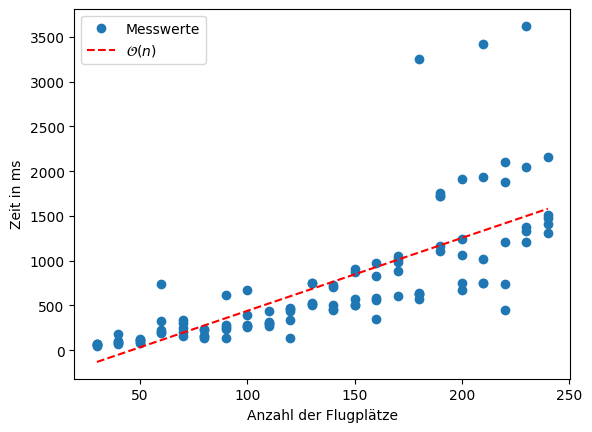
\includegraphics[scale=.5]{feasibletrend.png}
  \centering
  \caption{Messergebnisse zusammen mit einer linearen Funktion.}
\end{figure}
\subsection{Simulated Annealing}
Es sei $n$ die Anzahl der Flugplätze in der Eingabe, $T_0$ die Starttemperatur,
$\alpha$ der Abkühlkoeffizient und $T_{min}$ die Mindesttemperatur. Die
Temperatur im Schritt $s$ ist dann $T_0\alpha^s=T$. Um die Anzahl der Schritte
zu erhalten, können wir die Gleichung für $T=T_{min}$ lösen:
\begin{align*}
  T_0\alpha^s & = T_{min}                            & |:T_0          \\
  \alpha^s    & = \frac{T_{min}}{T_0}                & |\log_{\alpha} \\
  s           & = \log_{\alpha}(\frac{T_{min}}{T_0})                  \\
\end{align*}
Die Zeit für einen einzelnen Schritt liegt in $\mathcal{O}(n)$, denn jeder der Permutationsoperatoren
und die Berechnung der Kosten einer Lösung können in linearer Zeit durchgeführt werden. Die Zeit liegt also in
$\mathcal{O}(n\log_{\alpha}(\frac{T_{min}}{T_0}))$. Es muss immer nur die aktuell beste Lösung und der aktuelle Kandidat
gespeichert werden, wodurch der Speicherverbrauch in $\mathcal{O}(n)$ liegt.
\subsection{Optimale Lösung}
Es sei $n$ die Anzahl der Flugplätze in der Eingabe. Wir haben
$\frac{n(n-1)}{2}$ binäre Variablen für die Kanten ($x$) und $n$ binäre
Variablen für die Enden ($y$). Im schlechtesten Fall muss der
Branch-and-Cut-Algorithmus alle $2^{\frac{n(n-1)}{2}+n}$ möglichen
Kombinationen von Lösungen durchprobieren \cite[653]{korte_2018}. Die Zeit
liegt deshalb in $\mathcal{O}(2^(n^2))$. Der Algorithmus arbeitet einen
Suchbaum ab. Dabei geht der Algorithmus zuerst in die Tiefe des Suchbaums.
Dadurch muss für jede Variable immer nur eine weitere Verzweigung auf einmal
gespeichert werden, der Speicherverbrauch liegt also in
$\mathcal{O}(\frac{n(n-1)}{2}+n) = \mathcal{O}(n^2)$. Allerdings gibt es
$2^n$ Teilmengen von $L = \{1,2,\ldots n\}$, wodurch es auch $\mathcal{O}(2^n)$
Subtour-Elimination-Constraints gibt. Da diese im schlechtesten Fall alle
gespeichert werden müssen und eine dieser Ungleichungen $\mathcal{O}(n)$
Variablen enthält, liegt der Speicherverbrauch im schlechtesten Fall in $\mathcal{O}(n2^n)$.
\section{Umsetzung}
Den Simulated-Annealing-Algorithmus habe ich in Java implementiert. Wenn das
Programm ausgeführt wird, muss der Pfad zur Eingabedatei mit den Koordinaten
der Landeplätze angegeben werden. Dann wird eine Lösung gesucht, wobei der
Fortschritt ausgegeben wird. Die Lösung wird zusammen mit den Kosten
ausgegeben. Die Lösung wird als Permutation der Indices der Landeplätze in der
Eingabedatei ausgegeben, beginnend bei 0. Die beiden Versionen
\lstinline|SimulatedAnnealing.java| und
\lstinline|SimulatedAnnealingFeasible.java| unterscheiden sich darin, dass
letzteres den Algorithmus zum Finden einer beliebig teuren möglichen Lösung
implementiert. Ersteres speichert die Lösung zusätzlich in der Datei
\lstinline|<Eingabedatei>.solution|, damit das Ergebnis auch von der
Integer-Programming-Lösung verwendet werden kann. \\ Die
Integer-Programming-Lösung habe ich in Python implementiert. Dabei habe ich die
Bibliothek \lstinline|python-mip| verwendet, welche Mixed-Integer-Programme mit
dem CBC-Löser\cite{john_forrest_2023_7820266} löst. Für die Graph-Algorithmen,
also die Suche nach Zyklen und den Stoer-Wagner-Algorithmus, habe ich die
Bibliothek \lstinline|networkx| verwendet. Um eine Startlösung für den
CBC-Löser zu finden, wird die Java-Implementierung des
Simulated-Annealing-Algorithmus aufgerufen. Wenn das Programm ausgeführt wird,
muss auch hier der Pfad zur Lösung angegeben werden. Danach muss angegeben
werden, um wieviel Prozent die Lösung maximal von der optimalen Lösung
abweichen darf. Nach der Eingabe wird der Löser gestartet und gibt seinen
Fortschritt aus. Wenn der Löser fertig ist, wird auch hier eine Permutation der
Lösung ausgegeben.

\section{Beispiele}
Es handelt sich um die Beispiele von der BwInf-Webseite. Die Dateien sind im
Ordner \lstinline|beispiele| zu finden.
\subsection{Simulated Annealing: Beliebige gültige Lösung}
Eingabe: \lstinline|wenigerkrumm1.txt| \\ Ausgabe:
\begin{lstlisting}
Kosten: 2877.57
[50, 18, 33, 39, 54, 51, 0, 25, 21, 74, 73, 31, 47, 20, 36, 40, 83, 48, 77, 60, 68, 61, 
5, 55, 57, 23, 32, 22, 76, 12, 3, 42, 19, 75, 62, 41, 2, 17, 15, 56, 69, 82, 28, 35, 13, 
10, 6, 72, 81, 14, 7, 16, 4, 37, 38, 79, 53, 63, 34, 9, 70, 26, 52, 59, 71, 8, 80, 49, 
29, 11, 67, 58, 66, 1, 24, 27, 43, 44, 46, 30, 65, 64, 45, 78]
\end{lstlisting}
Eingabe: \lstinline|wenigerkrumm2.txt| \\ Ausgabe:
\begin{lstlisting}
Kosten: 7881.85
[39, 56, 40, 5, 29, 34, 31, 19, 27, 28, 15, 57, 45, 48, 51, 7, 26, 53, 38, 46, 24, 13, 
21, 20, 23, 22, 11, 10, 49, 1, 44, 50, 6, 25, 52, 37, 9, 47, 32, 4, 3, 42, 43, 16, 2, 
58, 35, 8, 14, 0, 41, 18, 59, 55, 33, 54, 12, 17, 30, 36]
\end{lstlisting}
Eingabe: \lstinline|wenigerkrumm3.txt| \\ Ausgabe:
\begin{lstlisting}
Kosten: 7677.73
[70, 42, 53, 41, 23, 4, 69, 78, 102, 75, 48, 81, 61, 85, 3, 0, 34, 101, 98, 86, 9,
115, 2, 49, 17, 92, 16, 73, 51, 27, 24, 87, 55, 29, 13, 26, 119, 74, 20, 43, 18, 90,
33, 22, 107, 97, 110, 114, 8, 38, 103, 68, 40, 99, 108, 59, 58, 32, 95, 54, 31, 93, 
105, 72, 36, 63, 46, 1, 113, 64, 5, 76, 94, 62, 77, 88, 112, 10, 71, 89, 80, 66, 
104, 106, 6, 111, 47, 84, 44, 60, 15, 57, 118, 56, 50, 28, 83, 21, 65, 45, 96, 117, 
7, 30, 116, 82, 14, 39, 79, 12, 25, 109, 35, 11, 91, 37, 19, 52, 100, 67]
\end{lstlisting}
Eingabe: \lstinline|wenigerkrumm4.txt| \\ Ausgabe:
\begin{lstlisting}
Kosten: 2500.85
[16, 0, 2, 9, 21, 1, 12, 6, 11, 7, 10, 5, 4, 8, 15, 14, 23, 22, 17, 19, 24, 13, 
20, 18, 3]
\end{lstlisting}
Eingabe: \lstinline|wenigerkrumm5.txt| \\ Ausgabe:
\begin{lstlisting}
Kosten: 8508.21
[57, 13, 59, 42, 30, 47, 37, 31, 39, 49, 14, 51, 48, 0, 46, 25, 18, 55, 1, 11, 24,
19, 52, 7, 26, 53, 22, 36, 2, 4, 35, 10, 29, 16, 54, 50, 8, 6, 12, 40, 44, 5, 41, 
33, 38, 15, 32, 27, 43, 21, 9, 45, 20, 3, 34, 23, 58, 28, 17, 56]
\end{lstlisting}
Eingabe: \lstinline|wenigerkrumm6.txt| \\ Ausgabe:
\begin{lstlisting}
Kosten: 8257.13
[69, 68, 77, 4, 29, 57, 15, 67, 37, 66, 48, 73, 49, 63, 45, 79, 50, 72, 6, 8, 40, 
20, 21, 78, 13, 3, 43, 33, 2, 16, 31, 56, 5, 74, 28, 75, 53, 47, 55, 52, 0, 18, 51,
41, 44, 24, 9, 36, 71, 19, 12, 17, 30, 27, 25, 11, 26, 46, 70, 60, 39, 64, 14, 34,
42, 32, 35, 61, 7, 59, 62, 54, 23, 58, 1, 10, 22, 65, 38, 76]
\end{lstlisting}
Eingabe: \lstinline|wenigerkrumm7.txt| \\ Ausgabe:
\begin{lstlisting}
Kosten: 12221.77
[21, 63, 22, 69, 27, 16, 65, 36, 73, 82, 71, 57, 93, 64, 53, 30, 40, 35, 99, 89,
72, 94, 80, 4, 17, 74, 3, 91, 66, 58, 0, 98, 24, 60, 79, 6, 28, 90, 46, 37, 68,
62, 86, 70, 7, 83, 67, 10, 77, 76, 75, 50, 48, 81, 87, 34, 15, 39, 29, 25, 85, 
59, 19, 55, 96, 12, 52, 44, 43, 13, 8, 95, 92, 49, 42, 41, 14, 97, 23, 84, 1, 
18, 78, 54, 11, 33, 61, 51, 88, 32, 9, 20, 2, 38, 31, 47, 56, 5, 26, 45]
\end{lstlisting}
\subsection{Simulated Annealing: Gute Lösung}
Eingabe: \lstinline|wenigerkrumm1.txt| \\ Ausgabe:
\begin{lstlisting}
Kosten: 847.43
[31, 19, 42, 73, 7, 16, 44, 46, 3, 30, 24, 12, 65, 64, 45, 41, 78, 76, 58, 67,
11, 2, 22, 29, 32, 49, 17, 23, 57, 48, 77, 60, 80, 68, 82, 69, 61, 8, 71, 59,
52, 50, 26, 18, 33, 70, 5, 56, 9, 34, 63, 55, 53, 39, 54, 15, 28, 51, 35, 79,
38, 37, 0, 4, 25, 13, 66, 1, 21, 83, 10, 74, 6, 40, 27, 72, 43, 81, 14, 36, 
62, 75, 20, 47]
\end{lstlisting}
Eingabe: \lstinline|wenigerkrumm2.txt| \\ Ausgabe:
\begin{lstlisting}
Kosten: 2183.66
[55, 59, 15, 9, 46, 10, 41, 0, 57, 37, 11, 22, 12, 19, 45, 48, 54, 25, 51, 7, 21,
3, 35, 4, 13, 44, 1, 49, 47, 24, 40, 5, 36, 29, 18, 38, 34, 30, 31, 16, 17, 43,
52, 14, 23, 27, 20, 42, 39, 8, 6, 26, 50, 53, 58, 33, 32, 2, 28, 56]
\end{lstlisting}
Eingabe: \lstinline|wenigerkrumm3.txt| \\ Ausgabe:
\begin{lstlisting}
Kosten: 1848.53
[67, 15, 113, 32, 102, 42, 14, 110, 1, 97, 53, 46, 58, 59, 108, 107, 22, 39, 91, 
79, 63, 2, 33, 37, 45, 96, 117, 49, 74, 25, 20, 109, 105, 35, 19, 48, 72, 36, 23,
16, 73, 86, 38, 10, 44, 54, 100, 43, 29, 55, 62, 77, 69, 84, 88, 116, 112, 28, 13, 
5, 61, 83, 21, 60, 26, 51, 9, 65, 115, 75, 41, 99, 119, 12, 40, 68, 103, 71, 11, 
52, 76, 94, 31, 81, 4, 92, 17, 93, 98, 101, 7, 89, 80, 30, 66, 104, 90, 18, 106, 6, 111, 
47, 50, 87, 56, 24, 118, 57, 34, 0, 3, 85, 82, 114, 78, 27, 70, 8, 64, 95]
\end{lstlisting}
Eingabe: \lstinline|wenigerkrumm4.txt| \\ Ausgabe:
\begin{lstlisting}
Kosten: 1205.07
[3, 1, 18, 14, 12, 23, 6, 11, 22, 17, 7, 19, 16, 0, 24, 13, 10, 5, 20, 4, 8, 2, 9, 15, 21]
\end{lstlisting}
Eingabe: \lstinline|wenigerkrumm5.txt| \\ Ausgabe:
\begin{lstlisting}
Kosten: 3257.92
[57, 54, 39, 32, 26, 7, 52, 31, 17, 34, 19, 24, 23, 38, 58, 28, 15, 53, 33, 50, 22, 37, 
47, 36, 2, 4, 41, 5, 20, 0, 48, 45, 42, 44, 59, 40, 12, 6, 13, 3, 8, 25, 46, 56, 30, 35, 
10, 51, 29, 18, 14, 9, 21, 43, 27, 11, 1, 49, 55, 16]
\end{lstlisting}
Eingabe: \lstinline|wenigerkrumm6.txt| \\ Ausgabe:
\begin{lstlisting}
Kosten: 3509.52
[55, 47, 77, 4, 49, 70, 60, 73, 52, 24, 6, 76, 44, 25, 38, 59, 67, 31, 56, 5, 20, 21,
12, 19, 37, 26, 71, 11, 66, 34, 42, 32, 35, 41, 36, 3, 0, 43, 79, 17, 22, 18, 51, 13, 
78, 10, 1, 74, 45, 28, 54, 23, 58, 40, 57, 15, 62, 65, 14, 16, 30, 64, 50, 48, 27, 72, 
61, 7, 39, 9, 2, 33, 46, 29, 75, 63, 8, 53, 69, 68]
\end{lstlisting}
Eingabe: \lstinline|wenigerkrumm7.txt| \\ Ausgabe:
\begin{lstlisting}
Kosten: 4397.65
[53, 50, 79, 43, 2, 65, 25, 84, 20, 77, 73, 36, 45, 26, 5, 94, 57, 75, 63, 40, 78, 86, 
19, 18, 51, 42, 41, 85, 72, 71, 1, 66, 35, 88, 32, 99, 89, 9, 82, 76, 59, 58, 21, 62, 
49, 30, 55, 69, 92, 22, 0, 61, 6, 93, 80, 14, 33, 28, 70, 56, 7, 96, 95, 98, 17, 34, 90, 
47, 81, 8, 13, 3, 10, 48, 15, 39, 64, 4, 97, 12, 23, 52, 44, 16, 29, 91, 38, 31, 67, 27, 
60, 24, 74, 83, 87, 46, 37, 68, 11, 54]
\end{lstlisting}
\subsection{Optimale Lösung}
Die Ausgaben des CBC-Lösers wurden hier ausgelassen. \\ Eingabe:
\lstinline|wenigerkrumm1.txt \n 0| \\ Ausgabe:
\begin{lstlisting}
Kosten: 847.43
[20, 75, 62, 36, 14, 81, 43, 72, 27, 40, 6, 74, 10, 83, 21, 1, 66, 13, 25, 4, 0, 37, 38, 
79, 35, 51, 28, 15, 54, 39, 53, 55, 63, 34, 9, 56, 5, 70, 33, 18, 26, 50, 52, 59, 71, 8, 
61, 69, 82, 68, 80, 60, 77, 48, 57, 23, 17, 49, 32, 29, 22, 2, 11, 67, 58, 76, 78, 41, 
45, 64, 65, 12, 24, 30, 3, 46, 44, 16, 7, 73, 42, 19, 31, 47]
\end{lstlisting}
Eingabe: \lstinline|wenigerkrumm2.txt \n 0| \\ Ausgabe:
\begin{lstlisting}
Kosten: 2183.66
[55, 59, 15, 9, 46, 10, 41, 0, 57, 37, 11, 22, 12, 19, 45, 48, 54, 25, 51, 7, 21,
3, 35, 4, 13, 44, 1, 49, 47, 24, 40, 5, 36, 29, 18, 38, 34, 30, 31, 16, 17, 43,
52, 14, 23, 27, 20, 42, 39, 8, 6, 26, 50, 53, 58, 33, 32, 2, 28, 56]
\end{lstlisting}
Eingabe: \lstinline|wenigerkrumm3.txt \n 0| \\ Ausgabe:
\begin{lstlisting}
Kosten: 1848.53
[67, 15, 113, 32, 102, 42, 14, 110, 1, 97, 53, 46, 58, 59, 108, 107, 22, 39, 91, 
79, 63, 2, 33, 37, 45, 96, 117, 49, 74, 25, 20, 109, 105, 35, 19, 48, 72, 36, 23,
16, 73, 86, 38, 10, 44, 54, 100, 43, 29, 55, 62, 77, 69, 84, 88, 116, 112, 28, 13, 
5, 61, 83, 21, 60, 26, 51, 9, 65, 115, 75, 41, 99, 119, 12, 40, 68, 103, 71, 11, 
52, 76, 94, 31, 81, 4, 92, 17, 93, 98, 101, 7, 89, 80, 30, 66, 104, 90, 18, 106, 6, 111, 
47, 50, 87, 56, 24, 118, 57, 34, 0, 3, 85, 82, 114, 78, 27, 70, 8, 64, 95]
\end{lstlisting}
Eingabe: \lstinline|wenigerkrumm4.txt \n 0| \\ Ausgabe:
\begin{lstlisting}
Kosten: 1205.07
[3, 1, 18, 14, 12, 23, 6, 11, 22, 17, 7, 19, 16, 0, 24, 13, 10, 5, 20, 4, 8, 2, 9, 15, 21]
\end{lstlisting}
Eingabe: \lstinline|wenigerkrumm5.txt \n 0| \\ Ausgabe:
\begin{lstlisting}
Kosten: 3257.92
[57, 54, 39, 32, 26, 7, 52, 31, 17, 34, 19, 24, 23, 38, 58, 28, 15, 53, 33, 50, 22, 37, 
47, 36, 2, 4, 41, 5, 20, 0, 48, 45, 42, 44, 59, 40, 12, 6, 13, 3, 8, 25, 46, 56, 30, 35, 
10, 51, 29, 18, 14, 9, 21, 43, 27, 11, 1, 49, 55, 16]
\end{lstlisting}
Eingabe: \lstinline|wenigerkrumm6.txt \n 0| \\ Ausgabe:
\begin{lstlisting}
Kosten: 3509.52
[55, 47, 77, 4, 49, 70, 60, 73, 52, 24, 6, 76, 44, 25, 38, 59, 67, 31, 56, 5, 20, 21,
12, 19, 37, 26, 71, 11, 66, 34, 42, 32, 35, 41, 36, 3, 0, 43, 79, 17, 22, 18, 51, 13, 
78, 10, 1, 74, 45, 28, 54, 23, 58, 40, 57, 15, 62, 65, 14, 16, 30, 64, 50, 48, 27, 72, 
61, 7, 39, 9, 2, 33, 46, 29, 75, 63, 8, 53, 69, 68]
\end{lstlisting}
Eingabe: \lstinline|wenigerkrumm7.txt \n 0| \\ Ausgabe:
\begin{lstlisting}
Kosten: 4150.64
[30, 55, 54, 11, 68, 37, 46, 87, 90, 83, 24, 60, 27, 67, 31, 38, 91, 29, 16, 39, 15, 48,
10, 3, 13, 8, 81, 47, 74, 17, 34, 7, 56, 70, 28, 33, 14, 6, 93, 80, 12, 97, 4, 50, 23, 
52, 44, 26, 45, 36, 73, 77, 20, 72, 84, 25, 65, 2, 43, 79, 64, 53, 98, 95, 96, 69, 92, 
22, 49, 0, 61, 75, 57, 94, 5, 85, 41, 42, 51, 59, 35, 88, 32, 99, 89, 9, 82, 71, 1, 66, 
76, 58, 21, 86, 78, 40, 63, 18, 19, 62]
\end{lstlisting}
\section{Quellcode}
\lstinputlisting[language=Java]{SimulatedAnnealing.java}
\lstinline|SimulatedAnnealingFeasible.java| ist in den Zeilen davor identisch zu \lstinline|SimulatedAnnealing.java|.
\lstinputlisting[language=Java,firstline=238]{SimulatedAnnealingFeasible.java}
\lstinputlisting[language=Python]{miptour.py}
\bibliographystyle{alpha}
\begingroup
\def\chapter*#1{}
\bibliography{refs.bib}
\endgroup
\end{document}